\begin{figure}[htp]
  \centering
  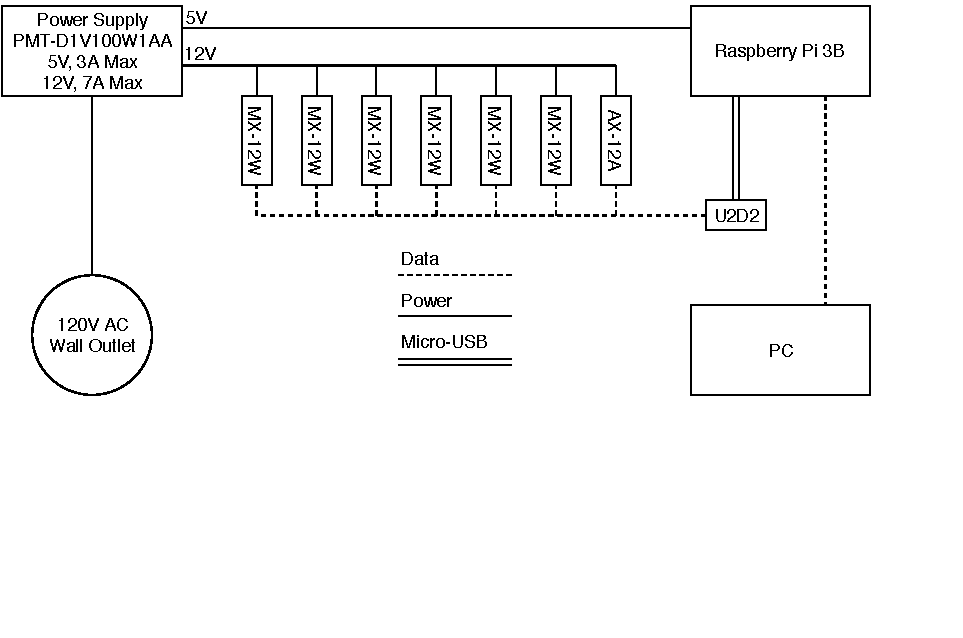
\includegraphics[width=.95\textwidth]{eschem}
  \caption{Electrical Block Diagram}
  \label{fig:ElectricalBlockDiagram}
\end{figure}
The electrical schematic shown in Figure \ref{fig:ElectricalBlockDiagram} consists of two power supplies that receive 120V AC supplied from wall outlets. The first power supply is the Raspberry Pi power supply, which outputs 5.1V at a max current of 2.5A via micro-usb. The second power supply, the RPS-200-12-C, has a 12V terminal with a max current output of 16.7A. The Raspberry Pi 3B is powered by the 5V micro-usb supply, and since the max current draw from the Pi is 1.2A the maximum current draw from the terminal is not surpassed. The three MX-64T servos and three MX-12W servos used in the manipulator, as well as the AX-12A servo used in the end effector, are connected in parallel from the 6 port MX/RX power hub, which is connected to the RPS-200-12-C by a 2.1mm barrel connector. Since the MX-64T has a stall current of 4.1A, the MX-12W has a stall current of .6A and the AX-12A has a stall current of 1.5A, the maximum current draw is 15.6A, less than the 16.7A the supply can output. In order to communicate to the servos, a U2D2 communication converter is connected to the Raspberry Pi which creates a serial connection used by the servos, allowing the servos to be daisy-chained together. The output of the U2D2 is connected to the MX/RX power hub, allowing the first servo in the daisy chain to receive both input data and power from the MX/RX power hub. The Raspberry Pi also connects to an external PC so that the user can communicate with the Pi using a mouse, keyboard, and monitor.

\begin{table}[htp]
  \center
  \caption{ Electrical Parts List}
  \label{tab:ElectricalPartsList}
  \begin{tabular}{c|c|c|c|c}
  Part & Qty & Individual Price & Transaction Cost & Cost to MEIOSIS \\\hline
  Raspberry Pi 3B & 1 & \$34.95 & \$34.95 & \$34.95 \\
  RPi Power Supply & 1 & \$9.95 & \$9.95 & \$9.95 \\
  RPi SD Card & 1 & \$12.95 & \$12.95 & \$12.95 \\
  U2D2 & 1 & \$49.90 & \$49.90 & \$0 \\
  RPS-200-12-C* & 1 & \$56.55 & \$56.55 & \$56.55 \\
  MX/RX Power Hub & 1 & \$7.95 & \$7.95 & \$0 \\
  DC Male Barrel Cable* & 1 & \$1.24 & \$1.24 & \$1.24 \\
  & & Total Cost & \$173.49 & \$115.64 \\
  \end{tabular}
  \small{*: Not Yet Purchased}
\end{table}

The parts list in Table \ref{tab:ElectricalPartsList} shows the costs of all the electrical components, as well as the actual cost to MEIOSIS.
